\documentclass[9pt]{beamer}

\usetheme{metropolis}
\metroset{progressbar=frametitle}
\usepackage[absolute,overlay]{textpos}
\newcommand{\tikzmark}[1]{\tikz[remember picture] \node[coordinate] (#1) {#1};}
\usepackage{pgfpages}
% \setbeameroption{show notes on second screen}
\usepackage{multimedia}
\usepackage{booktabs}


\usepackage{subfig}
% To fix in old caption: https://tex.stackexchange.com/questions/426088/texlive-pretest-2018-beamer-and-subfig-collide
\makeatletter
\let\@@magyar@captionfix\relax
\makeatother
\usepackage[square]{natbib} % Bibliography, citing: [\citet{storm_nonlinear_2005}]
\usepackage[scale=2]{ccicons}

\usepackage{pgfplots}
\usepgfplotslibrary{dateplot}
\graphicspath{{Figures/}}
\graphicspath{{Videos/}}
\title{Image Analysis on Biopolymer Networks}
\subtitle{Characterization using graphs}
\author{\textbf{Pablo Hernandez-Cerdan} \emph{\newline \textit{Main Supervisor}:} Prof. \underline{M.A.K Williams}}
\date{Biophysics Meeting at Massey University -- \today}
\institute{PhD. Student \newline
  Institute of Fundamental Sciences, Massey University\newline
  MacDiarmid Institute for Advanced Materials and Nanotechnology\newline
  Riddet Institute\newline
  New Zealand
}
% \titlegraphic{\hfill
\includegraphics[height=1.5cm]{./logo.pdf}}
\begin{document}

\maketitle

\begin{frame}
  \frametitle{Table of Contents}
  \setbeamertemplate{section in toc}[sections numbered]
  % \tableofcontents[hideallsubsections]
  \tableofcontents[hideallsubsections]
\end{frame}

\section{Motivation: Role of network architecture}
\begin{frame}{Sources of Strain-Stiffening}
  \begin{itemize}
    \item \citep{storm_nonlinear_2005}: strain stiffening arises from non linearity of single chains.
      Under the assumption that the network is isotropic and homogeneous.
      What does happens under other architectures?
    \item  \citep{onck_alternative_2005}, at the same time an alternative explanation of strain stiffening arised exclusively from
      network connectivity and relative orientation of the fibers.
  \end{itemize}
\end{frame}
\begin{frame}{Strain-Stiffening: Validity of Affine Deformation approximation in semi-flexible polymers}
  \note{ \citep{wilhelm_elasticity_2003} \citep{onck_alternative_2005}}
  \begin{columns}[onlytextwidth]
    \column{0.5\textwidth}
    \only<1,3->{
      \begin{exampleblock}{Affine transformations valid when: }
        \footnotesize{\textbf<4->{In Homogeneous and Isotropic Network}}
        \begin{itemize}
          \item Stiff Chains
          \item Dense Networks
        \end{itemize}
      \footnotesize{\citep{wilhelm_elasticity_2003}}
      \end{exampleblock}
    }
    \only<2>{
      \begin{alertblock}{Non-Affine range when:}
        \footnotesize{In Homogeneous and Isotropic Network}
        \begin{itemize}
          \item Compliant Chains
          \item Coarse Networks
        \end{itemize}
        \footnotesize{\citep{wilhelm_elasticity_2003}}
      \end{alertblock}
    }
    \column{0.5\textwidth}
    \begin{figure}[htpb]
      \centering
      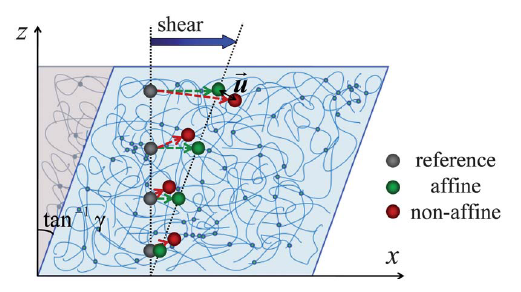
\includegraphics[width=0.9\textwidth]{./Figures/nonaffine.png}
      \caption*{\footnotesize{\citep{basu_nonaffine_2011, wen_non-affine_2012}}}
    \end{figure}
    \note{
      Difference between affine
      and non-affine deformation of a network under shear. Figure adopted from
      references
    }
  \end{columns}
  \only<2->{
  \begin{columns}[onlytextwidth]
    \column{0.5\textwidth}
    \begin{figure}[htpb]
      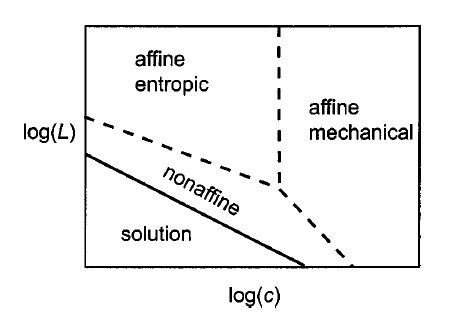
\includegraphics[width=0.7\textwidth]{./Figures/nonaffine-head.png}
      \caption*{\footnotesize{\textbf{L:} Molecular Weight, \textbf{c:} Concentration
      \citep{head_mechanical_2005}}}
    \end{figure}
    \only<3->{
      \column{0.5\textwidth}
      \begin{exampleblock}{Pre-stress and architecture role: }
        \footnotesize{
        Affine approx. is valid at constrained networks}
        \begin{itemize}
          \item Initial pre-stress constrains networks.
          \footnotesize{\citep{cioroianu_disorder_2015}}
          \item<4> Role of \textbf{Anisotropy} or \textbf{Architecture}?
        \end{itemize}
      \end{exampleblock}
    }
  \note{
    Molecular weight (L) and concentration (c). The solid line represents
    the rigidity percolation transition, where rigidity first appears at
    macroscopic level
  }
\end{columns}
}
\end{frame}
\begin{frame}
  \frametitle{Goals and research questions}
  % \metroset{block=fill}
  \begin{exampleblock}{}
  \begin{itemize}
    \item<1-> Going beyond the homogeneous and isotropic model of biopolymer networks: \textbf{Characterize the architecture} of connected filaments using images from different microscopy techniques depending on the size of the biopolymer.
    \item<2-> How different architectures do influent the \textbf{mechanical properties}? Are completely different biopolymers sharing similar geometries?
    \item<3-> Develop an open-source, free, user friendly, tested, and well documented software for others to use with microscopy images.
  \end{itemize}
  \end{exampleblock}
\end{frame}
\begin{frame}<beamer:0>
  \frametitle{The limit of the isotropic approximation}
  \begin{itemize}
    \item The power law behaviour has derived from universal slope of 1 \cite{mackintosh_bill} to \textbf{surprisingly(?)} a slope of  3/2. We think that this data require a further explanation beyond the assumption that collagen is somehow an exception in that universality claimed years ago.
    \item The shift to strain stiffening, or the beginning of a nematic phase of partially oriented fibers, might depend on architecture.
  \end{itemize}
\end{frame}
% \begin{frame}
%   \frametitle{Steps to characterize the network}
%   \begin{itemize}
%     \item Gathering the images. Microscopy.
%     \item Image analysis. Skeletonization.
%     \item Characterize the image with a graph representation.
%       \note
%       {
%         Grab the structure of a diluted enough network to be suceptible of the graph approach.
%         If it is too dense, probably the study of porosity would be more suitable
%       }
%   \end{itemize}
%       \begin{center}
%       \movie[height=0.4\textheight, width=0.65\textwidth, poster, autostart, loop]{}{./Videos/softwareShort.mp4}
%
%       \end{center}
% \end{frame}

\section{Gathering structure data:}

\begin{frame}
  \frametitle{Scattering: SAXS and SANS}
  \begin{itemize}
    \item Study of peaks and fractality at different q values provides an \textbf{averaged} structural information (mesh size, width of single-chains)
    \item It does not require special sample preparation.
    \item Good statistics, fast, allow study of dynamics.
    \item \alert{But}, it does not provide explicit 3D structure of exact connectivity.
  \end{itemize}
    \begin{figure}[htpb]
      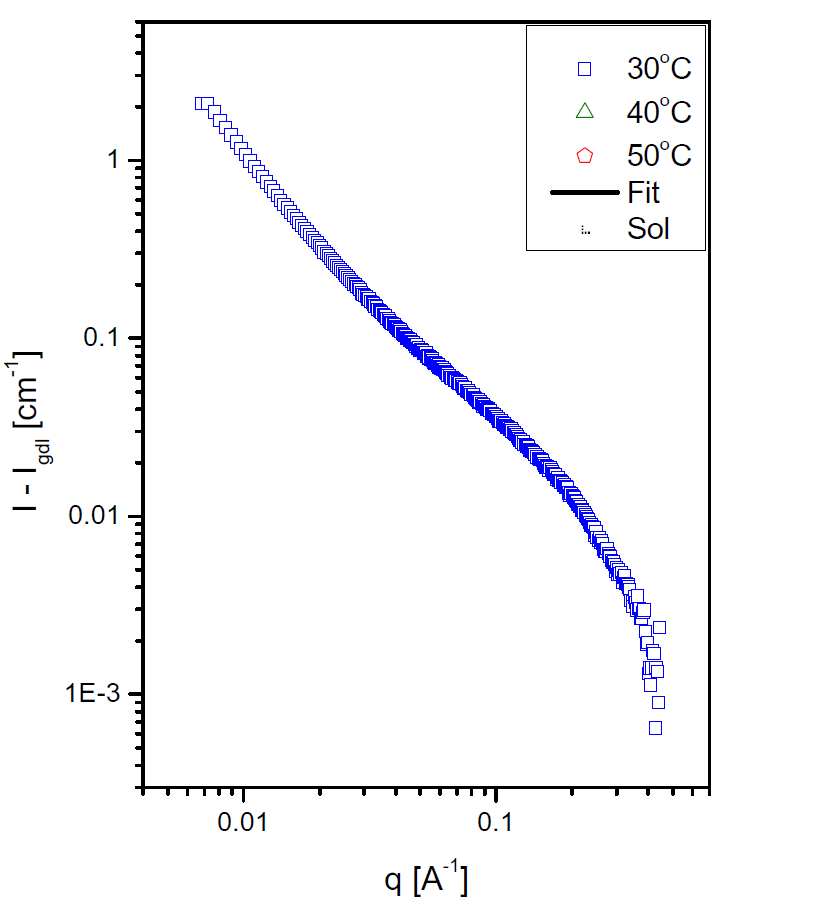
\includegraphics[width=0.25\textwidth]{./Figures/saxs_pectin.png}
      \caption*{\footnotesize{I vs q Pectin from SAXS}}
    \end{figure}
\end{frame}
\begin{frame}
  \frametitle{Microscopy: TEM and Confocal}
  To get detailed connectivity we need \textbf{3D microscopy}.
  \begin{columns}[T,onlytextwidth]
      \column{0.5\textwidth}
      \begin{exampleblock}{TEM tomography}
          \begin{itemize}
              \item Necessary to reach polysaccharides scale.
              \item Sample preparation is hard. Artifacts?
              \item \textbf{Working on validation method} comparing it with scattering.
          \end{itemize}
      \end{exampleblock}
      \column{0.5\textwidth}
      \begin{exampleblock}{Confocal}
          \begin{itemize}
              \item Suitable for most protein biopolymer networks.
              \item Sample preparation is more reliable.
          \end{itemize}
      \end{exampleblock}
  \end{columns}
  \begin{columns}[T,onlytextwidth]
  \column{0.5\textwidth}
      \centering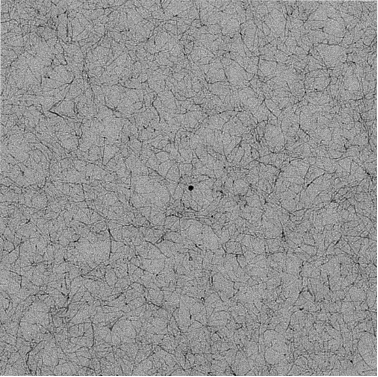
\includegraphics[width=0.5\textwidth]{./Figures/image_tem.png}
  \column{0.5\textwidth}
      \centering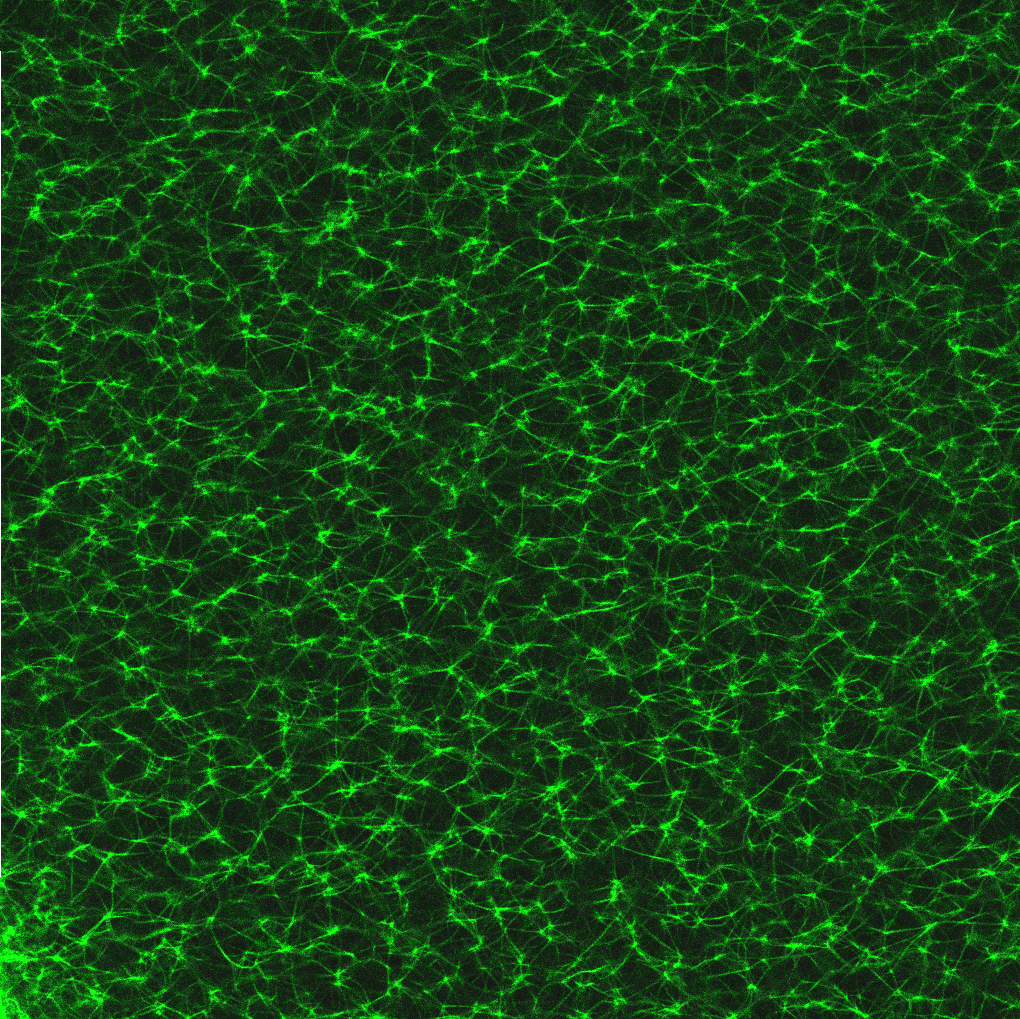
\includegraphics[width=0.5\textwidth]{./Figures/image_confocal.png}
  \end{columns}
\end{frame}

\section{Image Analysis}
\begin{frame}[t]
  \frametitle{Pipeline}
    \begin{alertblock}{Goal:}
        Process raw image data to get a spatial graph representation of the network.
    \end{alertblock}
    \vspace{0.8cm}
    \metroset{block=fill}
    \begin{exampleblock}{Steps:}
      \begin{enumerate}
        \item \textbf{Segmentation:} Extract object of interest from image. Binary image.
        \item \textbf{Skeletonization:} Thin representation of the object.
      \end{enumerate}
    \end{exampleblock}
    \vspace{1cm}
    The skeleton will then be adapted into a \textbf{Graph} for characterization.
    % \noindent\rule[0.1pt]{\linewidth}{0.01pt}
\end{frame}

\begin{frame}[t]
  \frametitle{Segmentation I}
    \alert{Goal:} Extract feature or region of interest from the raw image.

     Noise is the enemy.
     But also crowded environments from where only a specific feature is needed.

     \vspace{0.8cm}
     \metroset{block=fill}
     \begin{exampleblock}{Main Segmentation Methods:}
       \begin{itemize}
         \item \textbf{Threshold-Based:} Threshold at an intensity value. Entropy minimizing (Otsu) or other criteria.
         % \item \textbf{Region-Growing:} Local homogeneity of intensity criteria.
         \item \textbf{Enhancement Filter:} Local-phase studies or eigenvalue analysis of Hessian matrix.
         \item \textbf{Deformable-Model:} Curve evolving under vector field to fit structure. LevelSet (closed curve) or Snakes (open).
       \end{itemize}
     \end{exampleblock}
    % \noindent\rule[0.1pt]{\linewidth}{0.01pt}
\end{frame}

\begin{frame}[t]
  \frametitle{Segmentation in Confocal and TEM images of biopolymers}
     Need of preprocessing steps to reduce noise and enhance features of interest.
     \metroset{block=fill}
     \begin{exampleblock}{Pre-processing pipeline:}
     \begin{itemize}
       \item Multiscale characterization convolving image with gaussian operator of different sigmas/scales
       \item Denoise: Anisotropic edge-preserving filter.
       \item Enhancement Filter: Use a local-phase filter using a \textbf{monogenic-signal}, a N-D extension to the \textbf{analytic signal} used in modulation and demodulation of 1D communication signals.
     \end{itemize}
     \end{exampleblock}
     % \vspace{0.8cm}
    % \noindent\rule[0.1pt]{\linewidth}{0.01pt}
\end{frame}

\begin{frame}[t]
  \frametitle{Monogenic Signal: contribution to ITK}
    \begin{figure}[h]
      \centering
      
\includegraphics[height=1cm]{./Figures/software_logos/itkLogo.png}
      \caption*{Insight Toolkit: Registration and Segmentation}
    \end{figure}
    I am implementing a monogenic signal filter to ITK, the insight toolkit for image segmentation based on \citep{chenouard_3d_2011}.

    This filter applies operators in each direction of the FFT space, enhancing edge and line structures.
    It uses local phase information, and not absolute intensity, which helps detecting weak features.

    It is almost finished. I have to do the eigenanalysis to the filter and contribute (again) to this open source library.

    ITK is the main library for image analysis in C++, specially useful in segmentation of medical images and 3D stacks.
\end{frame}

\begin{frame}[t]
  \frametitle{Segmentation after the enhancement of the monogenic filter}
     After enhancement with the monogenic filter two options:
     \begin{itemize}
       \item The monogenic signal phase can be used to detect lines and edges. Use this measure to detect edges (more reliable than gradient or Sobel). Then use a level-set method, where the edge-measure is used to set the external vector field constraining the evolution \citep{rajpoot_local-phase_2009}.
       \item Exploit monogenic filter steering (rotation) properties. This allows to set an Eigensystem to find at each pixel the direction that maximizes the signal. Then threshold the enhanced image to get the segmentation \citep{chenouard_3d_2011}.
     \end{itemize}
\end{frame}

\begin{frame}[t]
  \frametitle{Skeletonization of segmented image}
     After segmentation, we have to thin the resulting binary object to a one-pixel wide representation that conserves topology.
     
     Skeletonization is really sensitive to noise in the borders, so a pruning is always required.
     \begin{columns}[T,onlytextwidth]
       \column{0.5\textwidth}
       \begin{exampleblock}{Global pruning:}
         \begin{itemize}
           \item It applies after the skeleton has been extracted.
           \item Only takes into account length of branches removing short but thin branches that might be significant for the architecture.
         \end{itemize}
       \end{exampleblock}
       \begin{figure}[h]
       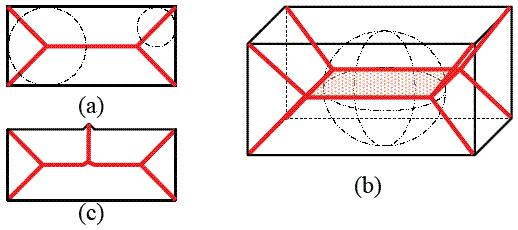
\includegraphics[height=2cm]{./Figures/skeleton/rectangle3D.jpg}
       \end{figure}
       \column{0.5\textwidth}
       \begin{exampleblock}{Local pruning:}
         \begin{itemize}
           \item Novel method to pruning at the same time than skeleton is generated.
           \item The pruning is made locally, thanks to a measure of \textbf{length of branch versus thickness.}
           \item It conserves short branches that are locally thin, but deletes short branches that are thick (see figure)
         \end{itemize}
       \end{exampleblock}
     \end{columns}
\end{frame}

\begin{frame}[t]
  \frametitle{Skeletonization: Cubical Complexes}
    \begin{figure}[h]
      \centering
      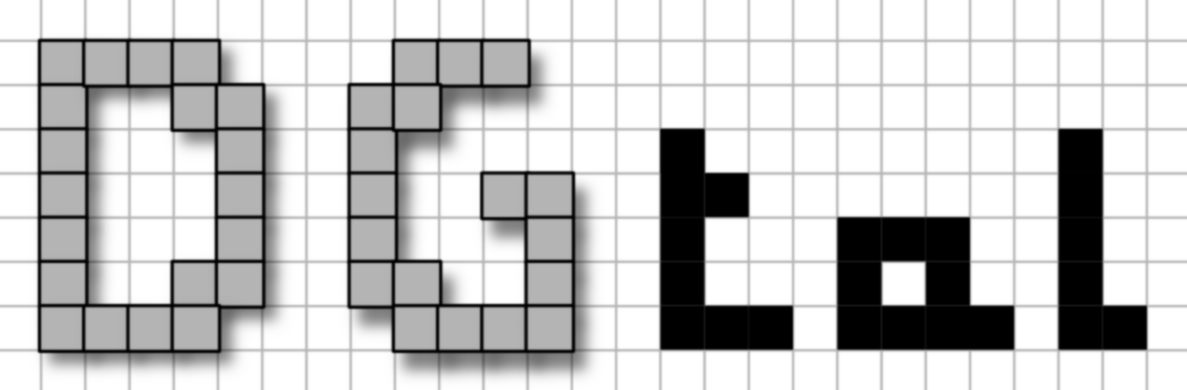
\includegraphics[height=1cm]{./Figures/software_logos/dgtalLogo.png}
      \caption*{DGTal:: Digital topology library}
    \end{figure}
    I have already contributed to DGtal the implementation of this local prune algorithm based on \citep{couprie_3d_2015}.

    And I am in the developing team!
    \begin{figure}[h]
      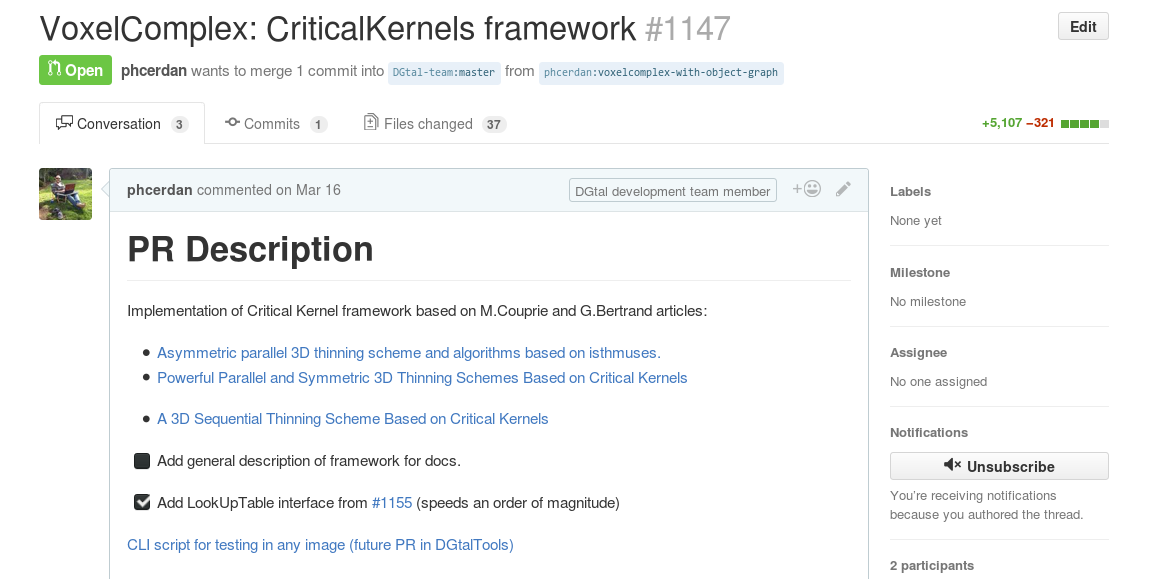
\includegraphics[width=0.6\textwidth]{./Figures/skeleton/dgtalGithub.png}
    \end{figure}
\end{frame}

\begin{frame}[t]
  \frametitle{Skeletonization: Cubical Complexes}
  \begin{columns}[T,onlytextwidth]
    \column{0.5\textwidth}
    \begin{exampleblock}{Global pruning:}
      \begin{itemize}
        \item Uses a framework called CubicalComplexes or VoxelComplexes, where a spel (voxel in 3D, pixel in 2D) is composed by points, lines and faces.
        \item This allow to define a topology property called Isthmus in all those components, that preserves topology in the skeletonization process.
        % \item The local prunning is made setting a life-time parameter, measuring the iterations between a pixel has been marked for removal (because its deletion doesn't change topology) and the iteration where it was definitely removed.
      \end{itemize}
    \end{exampleblock}
    \column{0.5\textwidth}
    \begin{figure}[h]
      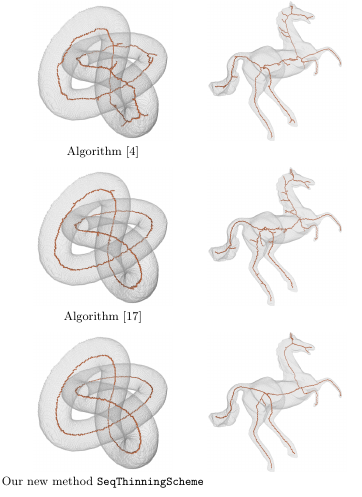
\includegraphics[width=0.9\textwidth]{./Figures/skeleton/thinningCouprie.png}
    \end{figure}
  \end{columns}
\end{frame}

\begin{frame}[t]
  \frametitle{Summary of image analysis}
  \begin{exampleblock}{Pipeline:}
    \begin{description}[<+-| alert@+>]
      \item<1->[Multiscale analysis and denoise:] Detect vessels of different radius.
      \item<2->[Segmentation:] Get a binary object that conserves features. 
      \item<3->[Skeletonization:] One-pixel wide (thin) representation of binary object, conserving topology.
      \item<4->[Graph adaptor:] Transform skeleton to a graph, to connect with ComplexSystems tools for characterization.
    \end{description}
  \end{exampleblock}
  \begin{textblock*}{2cm}(1.5cm,6.9cm) % {block width} (coords)
    \tikzmark{n1}
    \uncover<2->{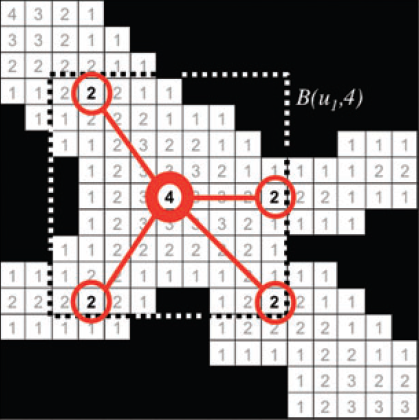
\includegraphics[width=2cm]{./Figures/fire/nucleation1.png}}
  \end{textblock*}
  \begin{textblock*}{1.5cm}(7.5cm,6.5cm)
    \tikzmark{t1}
    \uncover<3->{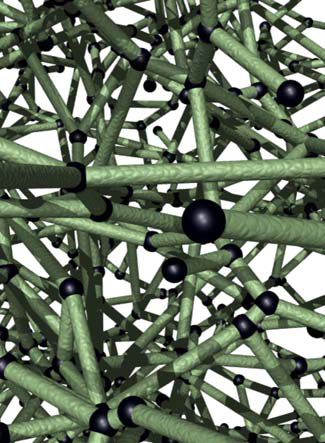
\includegraphics[width=1.5cm]{./Figures/skeleton/lind.png}}
  \end{textblock*}
  \begin{textblock*}{2cm}(9.1cm,7cm)
    \uncover<4->{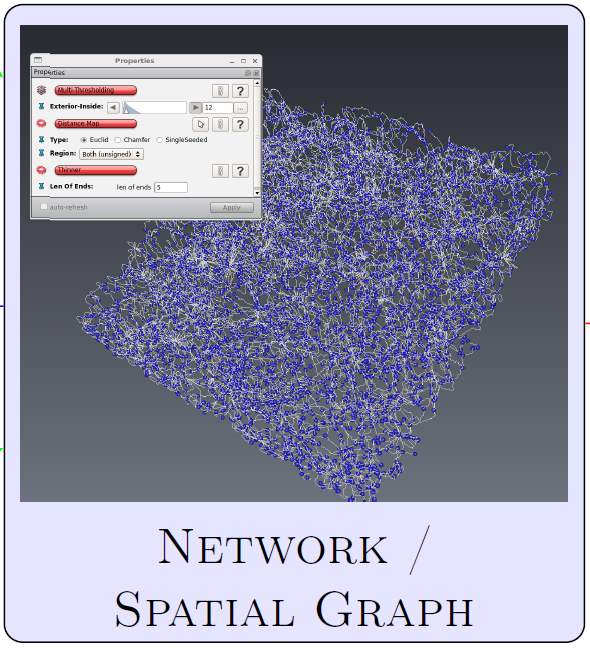
\includegraphics[width=2cm]{./Figures/skeleton/aviz.png}}
  \end{textblock*}
  \begin{tikzpicture}[remember picture,overlay]
    %\path[draw=magenta,thick,->]<3-> ([yshift=3mm]n1) to ++(0,3mm) to [out=0, in=0,distance=2.5in] (t1);
    \path[draw=green,thick,->]<3-> ([xshift=2.2cm, yshift=-1cm]n1) -- ([xshift=-0.2cm,yshift=-1.4cm]t1);
  \end{tikzpicture}
\end{frame}

\section{Graph Characterization}
\begin{frame}
  \frametitle{Graphs: A Link to Complex Systems}
  A graph is a representation of connected components in terms of nodes and edges/links.

  \begin{exampleblock}{Spatial Network of biopolymers:}
    \begin{itemize}
      \item A node corresponds to a junction/crosslink of biopolymers.
      \item An edge represents the polymer-chain itself.
    \end{itemize}
  \end{exampleblock}

  Graphs are a powerful tool connecting to the field of \textbf{Complex Systems}.

  We want to take advantage of all those existing algorithms for \textbf{characterization} of soft materials.

\end{frame}
\begin{frame}
  \frametitle{Graphs: A Link to Complex Systems}
  With a graph representation of the system we can now link our spatial graph to standard complex network libraries.
  \begin{description}[t]
      \item[IGraph] C, R, Python (GPL licence)
      \item[Boost: Graph and GraphParallel] C++ (MIT licence)
      \item[NetworkX] Python (MIT licence)
  \end{description}

  \vspace{1cm}
  \begin{columns}[onlytextwidth]
      \column{0.33\textwidth}
      
\includegraphics[width=0.9\textwidth]{./Figures/software_logos/igraph_tittle.png}
      \column{0.33\textwidth}
      
\includegraphics[width=0.9\textwidth]{./Figures/software_logos/boost_logo.jpeg}
      \column{0.33\textwidth}
      
\includegraphics[width=0.9\textwidth]{./Figures/software_logos/networkx_logo.jpeg}
  \end{columns}

\end{frame}
\begin{frame}
  \frametitle{Generating Software Tools}
  \begin{columns}[onlytextwidth]
      \column{0.49\textwidth}
      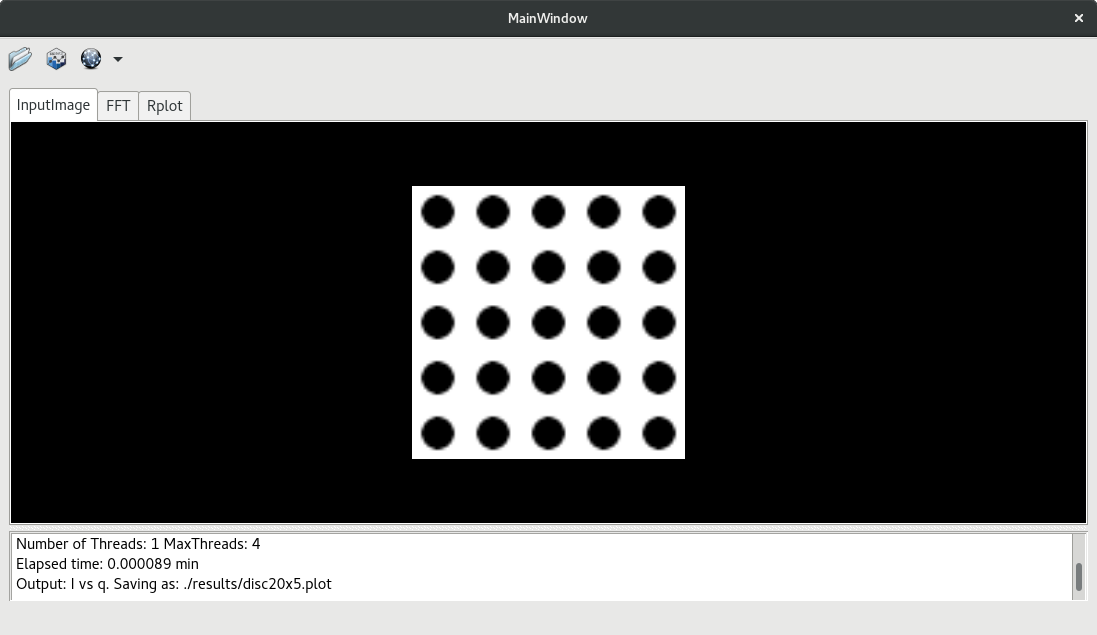
\includegraphics[width=0.9\textwidth]{./Figures/software_screenshots/fft_screenshot.png}
      \vspace{1cm}
      Radial FFT analysis to compare images and SAXS:
      \column{0.49\textwidth}
      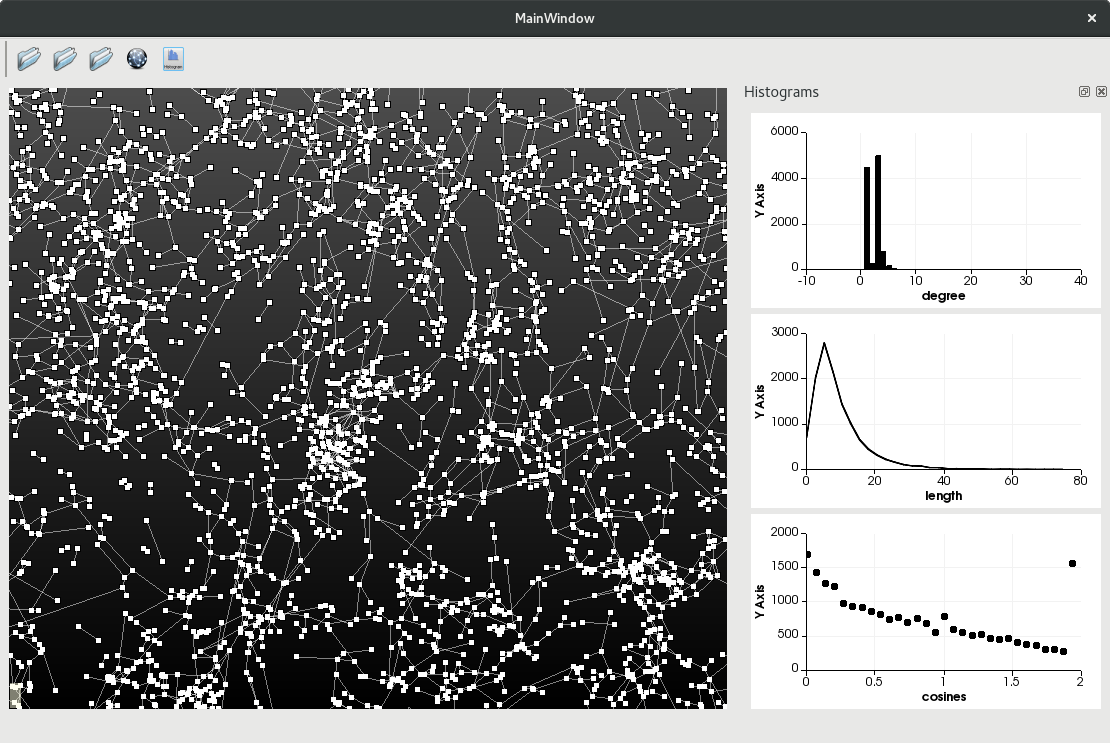
\includegraphics[width=0.9\textwidth]{./Figures/software_screenshots/graph_to_distrutions.png}
      \vspace{1cm}
      Compute statistical distributions from graph.
  \end{columns}
  % \centering
  % \movie[height=0.75\textheight, width=\textwidth, poster, autostart, loop, showcontrols]{}{Videos/softwareShort.mp4}
  \note
  {
    Instead of using a one time solution, I am interested in provide computational, user friendly tools for others to use.\newline
    This has driven me to the software development side
  }
\end{frame}

\begin{frame}
  \frametitle{Generating Software Tools II}
  \begin{columns}[onlytextwidth]
      \column{0.49\textwidth}
      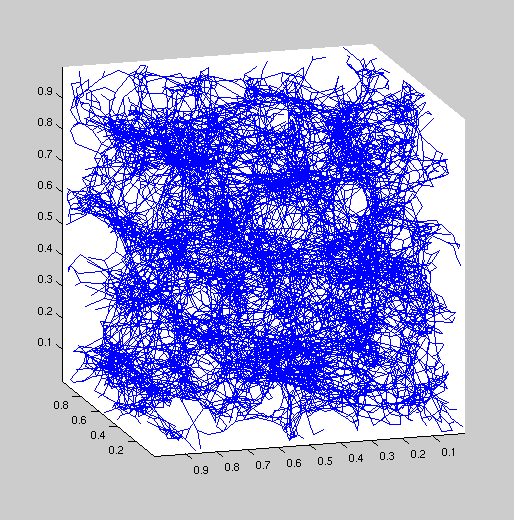
\includegraphics[width=0.9\textwidth]{./Figures/chapter-reconstruct/networkN10000.png}
      \vspace{1cm}
      Reconstruct in-silico network from graph statistical distributions
      %\citep{lindstrom_biopolymer_2010}:
      \column{0.49\textwidth}
      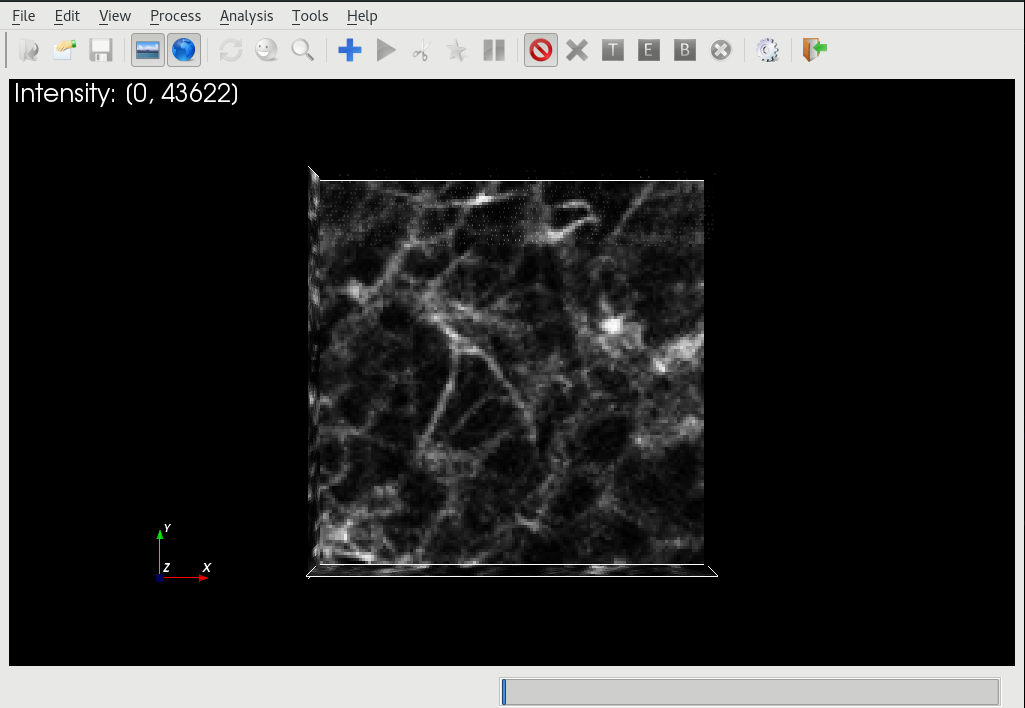
\includegraphics[width=0.9\textwidth]{./Figures/software_screenshots/sgext.png}
      \vspace{1cm}
      Not revelead yet (sorry!): Merge of software when segmentation is ready.

      SGEXT: Spatial Graph Extractor. Name suggestions welcome! (MAIDEN?)
      %\citep{lindstrom_biopolymer_2010}:
  \end{columns}
\end{frame}

% \begin{frame}
%   \frametitle{Results: Proof of concept}
%   \footnotesize{
%   \uncover<1>{Three Networks analyzed:
%   \begin{columns}[onlytextwidth]
%       \column{0.5\textwidth}
%       \begin{itemize}
%       \item Polysaccharides using TEM: Pectin, Carrageenan
%       \end{itemize}
%       \column{0.5\textwidth}
%       \begin{itemize}
%           \item Proteins using Confocal: Actin (Collagen from literature \citep{lindstrom_finite-strain_2013} ).
%       \end{itemize}
%   \end{columns}
%   }
%   \uncover<2->{
%       Statistical distributions of local graph properties:
%       \alert{Showing same functional forms}
%
%       \vspace{1mm}
%   }
%   }
%   \vspace{0.5cm}
%   \centering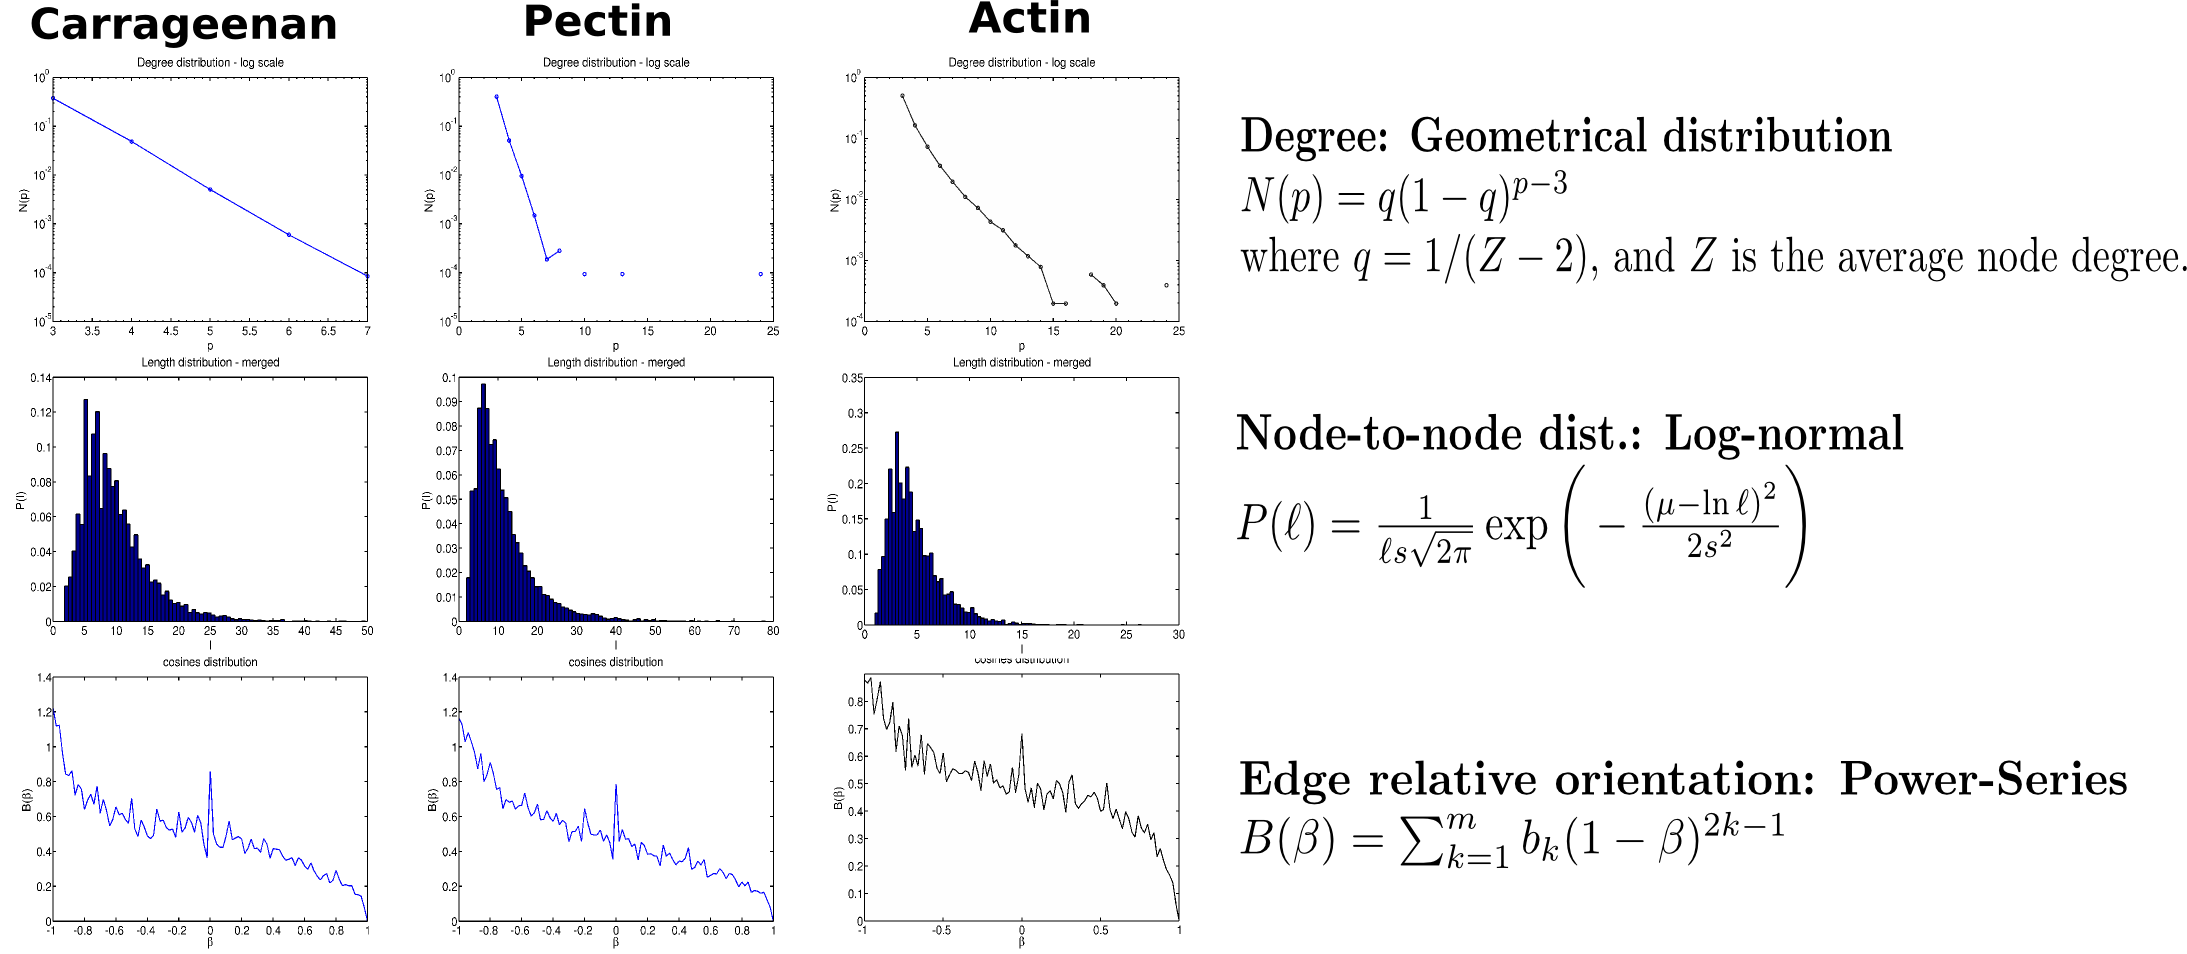
\includegraphics[width=0.99\textwidth]{./Figures/results_poster.png}
% \end{frame}
\begin{frame}
  \frametitle{Summary}
  \begin{columns}[onlytextwidth]
      \column{0.60\textwidth}
      \metroset{block=fill}
      \begin{alertblock}{Exploring network geometries:}
          \begin{itemize}
              \item When does architecture matter? What is its role at lower scales?
              \item Gather best image analysis techniques for biopolymers.
              \item Link to complex network libraries for graph analysis. \textbf{Reconstruct in-silico networks from it}
              \item \alert{The dream} would be to provide soft-matter scientists with a reliable tool to \textbf{characterize} their materials, linking to the field of ComplexSystems.
          \end{itemize}
      \end{alertblock}
      \column{0.40\textwidth}
        \centering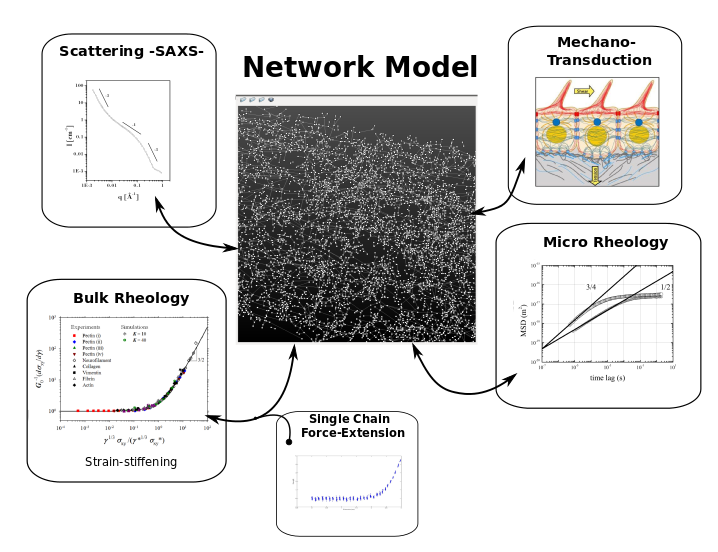
\includegraphics[width=\textwidth]{./Figures/network_model_fig.png}
  \end{columns}
\end{frame}
\begin{frame}{Acknowledgments}

  \vspace{0.3cm}
  \begin{columns}[onlytextwidth]
    \column{0.33\textwidth}
    
\includegraphics[width=0.9\textwidth]{./Figures/people/macdiarmid.png}
    \column{0.33\textwidth}
    
\includegraphics[width=0.9\textwidth]{./Figures/people/massey.png}
    \column{0.33\textwidth}
    
\includegraphics[width=0.9\textwidth]{./Figures/people/riddet.png}
  \end{columns}
  \begin{columns}[onlytextwidth]
    \column{0.5\textwidth}
\begin{figure}[htpb]
  \centering
  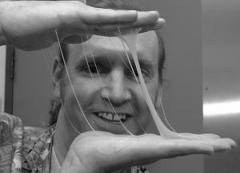
\includegraphics[width=0.8\textwidth]{./Figures/people/bill.png}
  \caption*{Main Supervisor: \textbf{Prof. M.A.K Williams}}
\end{figure}
    \column{0.5\textwidth}
    \begin{figure}[htpb]
      \centering
      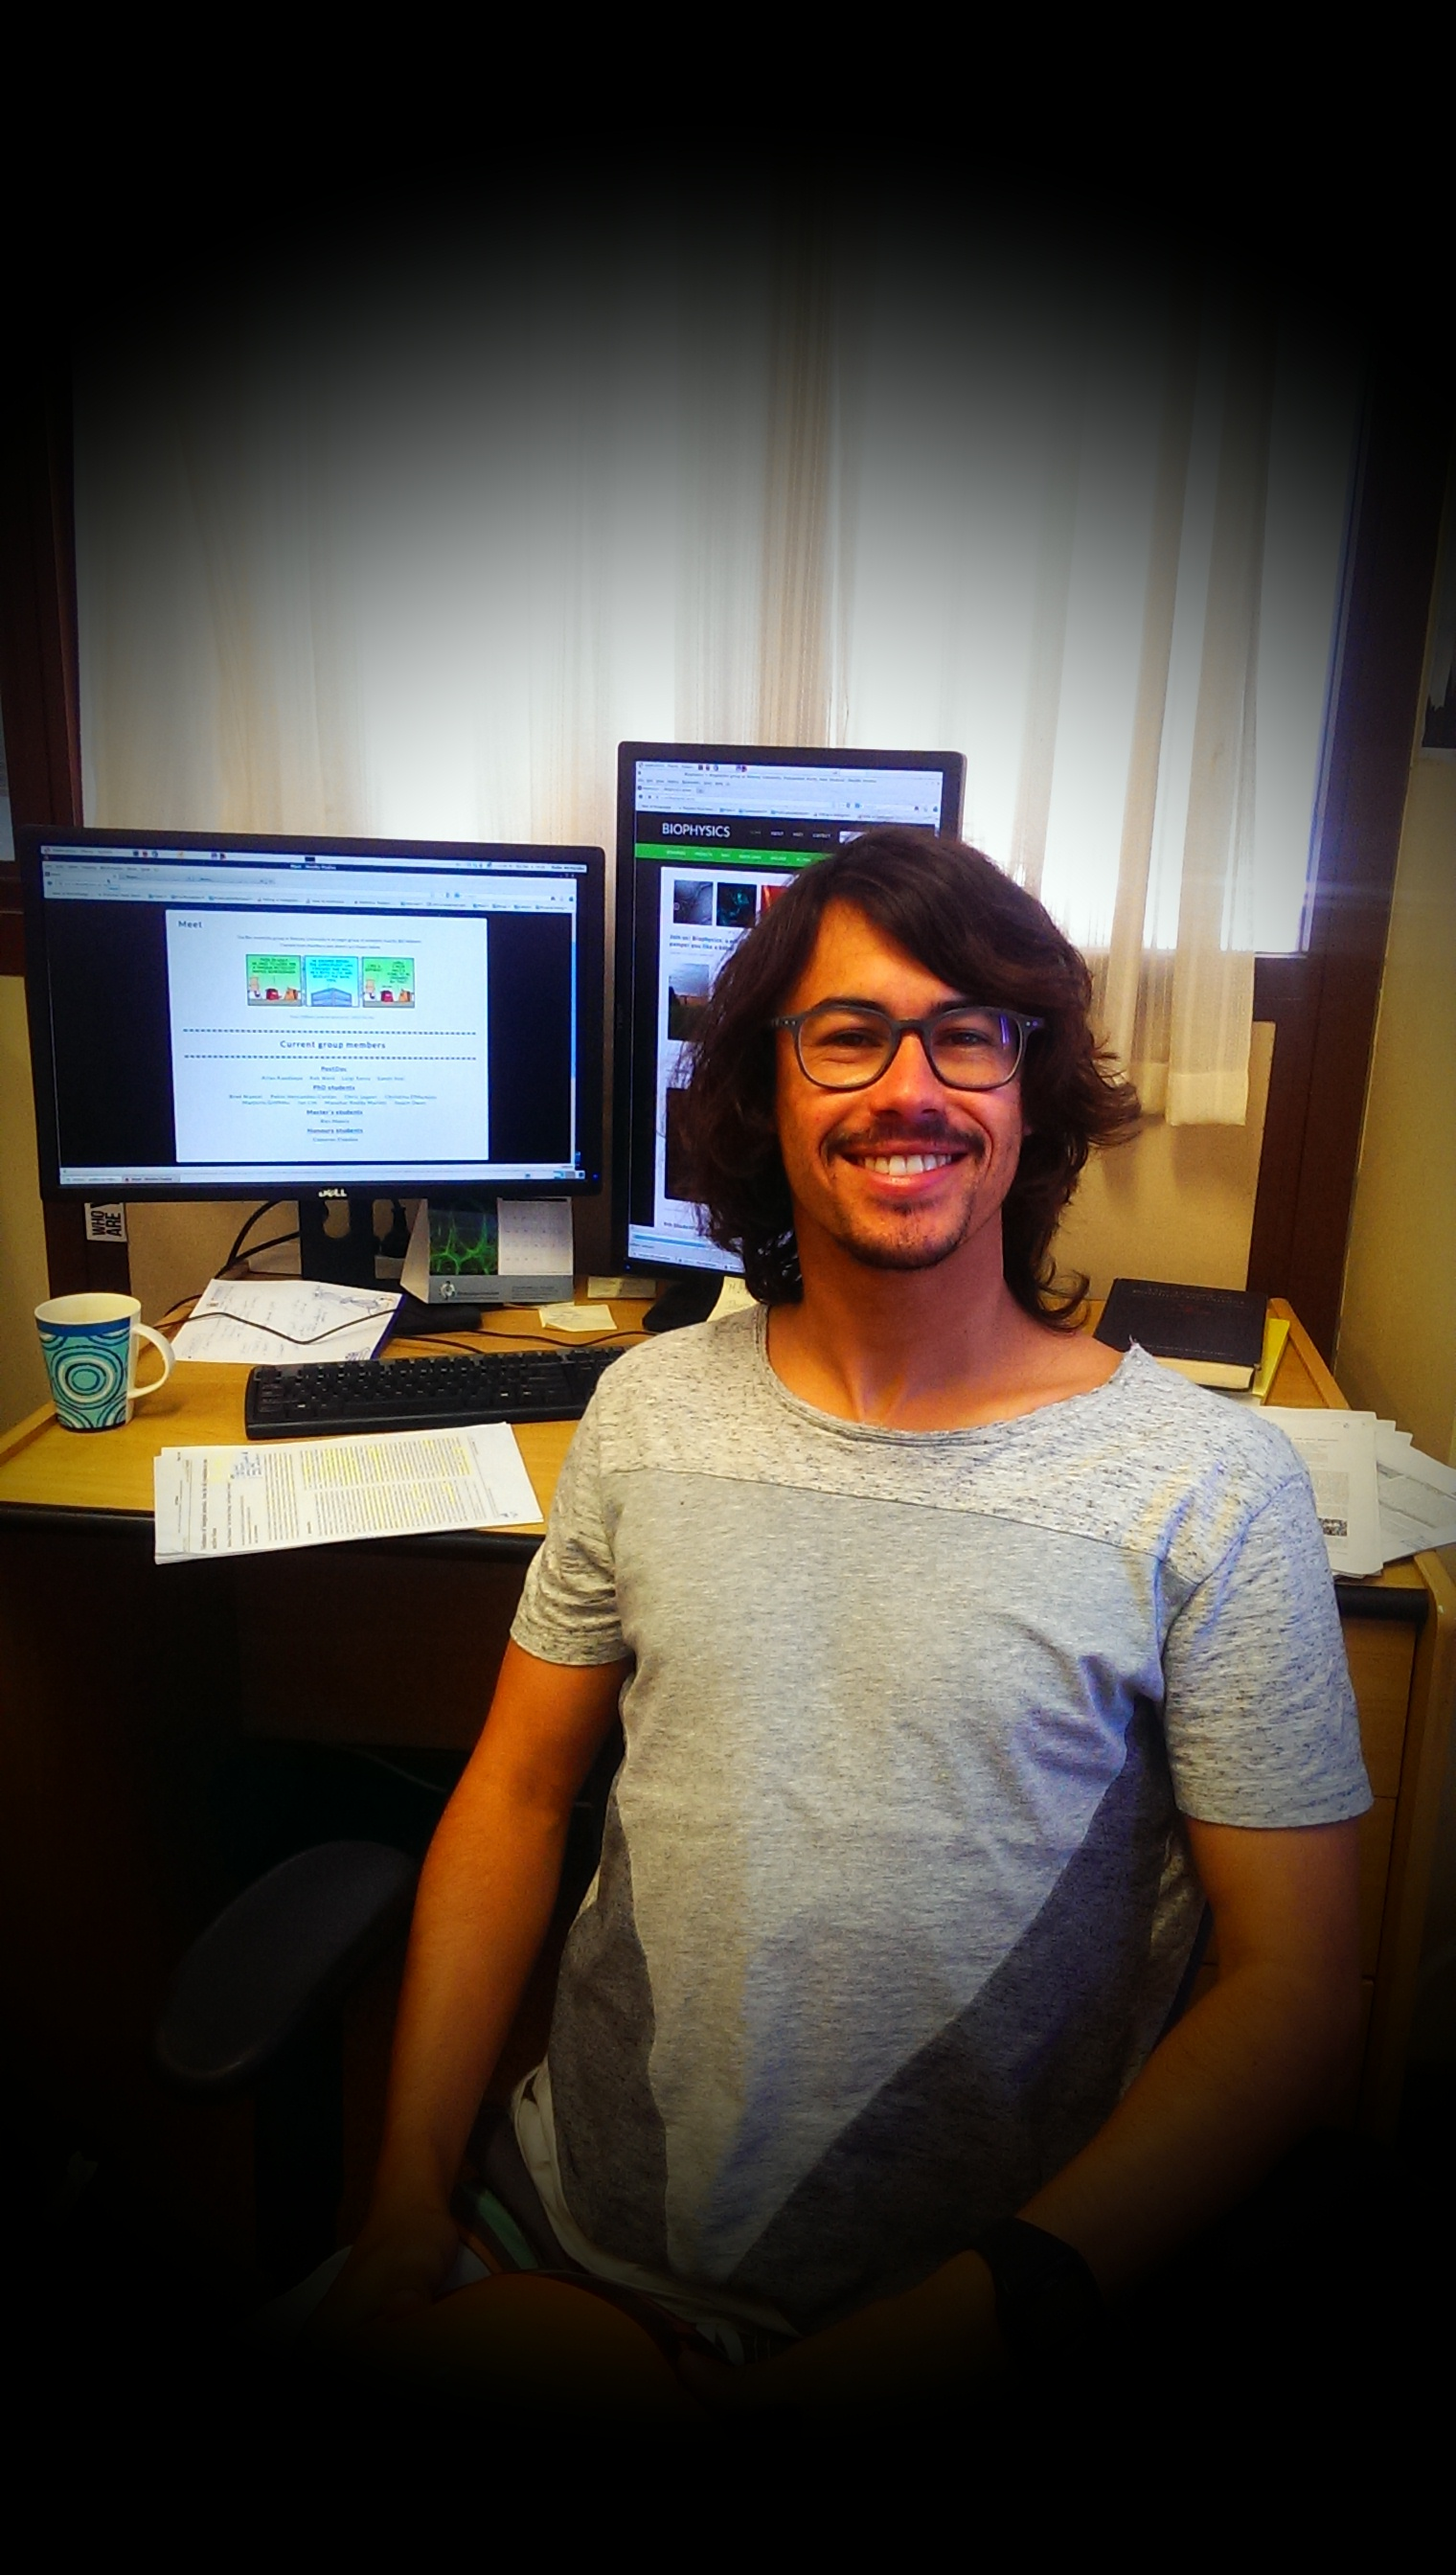
\includegraphics[width=0.3\textwidth]{./Figures/people/brad.png}
      \caption*{Dr. Brad Mansel, New Zealand}
    \end{figure}
  \end{columns}
  \begin{columns}[onlytextwidth]
    \column{0.45\textwidth}
    \begin{itemize}
      \item Andrew Leis. CSIRO Animal Health. Australia.
      \item Leif Lundin. SP Food and Bioscience. Sweden.
    \end{itemize}
    \column{0.45\textwidth}
    \textbf{Visit us in NZ or online at:}\newline
        \url{www.biophysics.ac.nz}
  \end{columns}
\end{frame}
\plain{Thanks for your attention!}
\begin{frame}{Follow development live in github}
  Keep up to date with further development at my github page:
  \vspace{2mm}
  \begin{columns}[onlytextwidth]
    \column{0.45\textwidth}
      \begin{center}\url{github.com/phcerdan}\end{center}
    \column{0.45\textwidth}
      \movie[height=0.3\textheight, width=0.8\textwidth, poster, autostart, loop]{}{Videos/softwareShort.mp4}
  \end{columns}


  \vspace{2mm}
  Get this beamer theme from:

  \begin{center}\url{github.com/matze/mtheme}\end{center}

  \begin{center}\ccbysa\end{center}

\end{frame}
\begin{frame}[allowframebreaks]

  \frametitle{References}

  \bibliography{bibliography}
  \bibliographystyle{plainnat}

\end{frame}

\end{document}

% \begin{frame}{Lists}
%   \begin{columns}[T,onlytextwidth]
%     \column{0.33\textwidth}
%       Items
%       \begin{itemize}
%         \item Milk \item Eggs \item Potatos
%       \end{itemize}

%     \column{0.33\textwidth}
%       Enumerations
%       \begin{enumerate}
%         \item First, \item Second and \item Last.
%       \end{enumerate}

%     \column{0.33\textwidth}
%       Descriptions
%       \begin{description}
%         \item[PowerPoint] Meeh. \item[Beamer] Yeeeha.
%       \end{description}
%   \end{columns}
% \end{frame}
% \begin{frame}{Animation}
%   \begin{itemize}[<+- | alert@+>]
%     \item \alert<4>{This is\only<4>{ really} important}
%     \item Now this
%     \item And now this
%   \end{itemize}
% \end{frame}
% \begin{frame}{Figures}
%   \begin{figure}
%     \newcounter{density}
%     \setcounter{density}{20}
%     \begin{tikzpicture}
%       \def\couleur{alerted text.fg}
%       \path[coordinate] (0,0)  coordinate(A)
%                   ++( 90:5cm) coordinate(B)
%                   ++(0:5cm) coordinate(C)
%                   ++(-90:5cm) coordinate(D);
%       \draw[fill=\couleur!\thedensity] (A) -- (B) -- (C) --(D) -- cycle;
%       \foreach \x in {1,...,40}{%
%           \pgfmathsetcounter{density}{\thedensity+20}
%           \setcounter{density}{\thedensity}
%           \path[coordinate] coordinate(X) at (A){};
%           \path[coordinate] (A) -- (B) coordinate[pos=.10](A)
%                               -- (C) coordinate[pos=.10](B)
%                               -- (D) coordinate[pos=.10](C)
%                               -- (X) coordinate[pos=.10](D);
%           \draw[fill=\couleur!\thedensity] (A)--(B)--(C)-- (D) -- cycle;
%       }
%     \end{tikzpicture}
%     \caption{Rotated square from
%     \href{http://www.texample.net/tikz/examples/rotated-polygons/}{texample.net}.}
%   \end{figure}
% \end{frame}
% \begin{frame}{Tables}
%   \begin{table}
%     \caption{Largest cities in the world (source: Wikipedia)}
%     \begin{tabular}{lr}
%       \toprule
%       City & Population\\
%       \midrule
%       Mexico City & 20,116,842\\
%       Shanghai & 19,210,000\\
%       Peking & 15,796,450\\
%       Istanbul & 14,160,467\\
%       \bottomrule
%     \end{tabular}
%   \end{table}
% \end{frame}
% \begin{frame}{Blocks}
%   Three different block environments are pre-defined and may be styled with an
%   optional background color.

%   \begin{columns}[T,onlytextwidth]
%     \column{0.5\textwidth}
%       \begin{block}{Default}
%         Block content.
%       \end{block}

%       \begin{alertblock}{Alert}
%         Block content.
%       \end{alertblock}

%       \begin{exampleblock}{Example}
%         Block content.
%       \end{exampleblock}

%     \column{0.5\textwidth}

%       \metroset{block=fill}

%       \begin{block}{Default}
%         Block content.
%       \end{block}

%       \begin{alertblock}{Alert}
%         Block content.
%       \end{alertblock}

%       \begin{exampleblock}{Example}
%         Block content.
%       \end{exampleblock}

%   \end{columns}
% \end{frame}
% \begin{frame}{Math}
%   \begin{equation*}
%     e = \lim_{n\to \infty} \left(1 + \frac{1}{n}\right)^n
%   \end{equation*}
% \end{frame}
% \begin{frame}{Line plots}
%   \begin{figure}
%     \begin{tikzpicture}
%       \begin{axis}[
%         mlineplot,
%         width=0.9\textwidth,
%         height=6cm,
%       ]

%         \addplot {sin(deg(x))};
%         \addplot+[samples=100] {sin(deg(2*x))};

%       \end{axis}
%     \end{tikzpicture}
%   \end{figure}
% \end{frame}
% \begin{frame}{Bar charts}
%   \begin{figure}
%     \begin{tikzpicture}
%       \begin{axis}[
%         mbarplot,
%         xlabel={Foo},
%         ylabel={Bar},
%         width=0.9\textwidth,
%         height=6cm,
%       ]

%       \addplot plot coordinates {(1, 20) (2, 25) (3, 22.4) (4, 12.4)};
%       \addplot plot coordinates {(1, 18) (2, 24) (3, 23.5) (4, 13.2)};
%       \addplot plot coordinates {(1, 10) (2, 19) (3, 25) (4, 15.2)};

%       \legend{lorem, ipsum, dolor}

%       \end{axis}
%     \end{tikzpicture}
%   \end{figure}
% \end{frame}

